\documentclass[12pt]{article}
\usepackage{amsthm,amssymb,amsfonts,amsmath,amstext,systeme}
\usepackage{graphicx,float}
\usepackage{tabularx}

\marginparwidth 0pt
\oddsidemargin -1.2 truecm
\evensidemargin  0pt 
\marginparsep 0pt
\topmargin -2.2truecm
\linespread{1}
\textheight 25.8 truecm
\textwidth 18.5 truecm
\newenvironment{remark}{\noindent{\bf Remark }}{\vspace{0mm}}
\newenvironment{remarks}{\noindent{\bf Remarks }}{\vspace{0mm}}
\newenvironment{question}{\noindent{\bf Question }}{\vspace{0mm}}
\newenvironment{questions}{\noindent{\bf Questions }}{\vspace{0mm}}
\newenvironment{note}{\noindent{\bf Note }}{\vspace{0mm}}
\newenvironment{summary}{\noindent{\bf Summary }}{\vspace{0mm}}
\newenvironment{back}{\noindent{\bf Background}}{\vspace{0mm}}
\newenvironment{conclude}{\noindent{\bf Conclusion}}{\vspace{0mm}}
\newenvironment{concludes}{\noindent{\bf Conclusions}}{\vspace{0mm}}
\newenvironment{dill}{\noindent{\bf Description of Dill's model}}{\vspace{0mm}}
\newenvironment{maths}{\noindent{\bf Mathematics needed}}{\vspace{0mm}}
\newenvironment{inst}{\noindent{\bf Instructions}}{\vspace{0mm}}
\newenvironment{notes}{\noindent{\bf Notes }}{\vspace{0mm}}
\newenvironment{theorem}{\noindent{\bf Theorem }}{\vspace{0mm}}
\newenvironment{example}{\noindent{\bf Example }}{\vspace{0mm}}
\newenvironment{examples}{\noindent{\bf Examples }}{\vspace{0mm}}
\newenvironment{topics}{\noindent{\bf Topics}}{\vspace{0mm}}
\newenvironment{outcomes}{\noindent{\bf Expected Learning Outcomes}}{\vspace{0mm}}
\newenvironment{lemma}{\noindent{\bf Lemma }}{\vspace{0mm}}
\newenvironment{solution}{\noindent{\it Solution}}{\vspace{2mm}}
\newcommand{\ds}{\displaystyle}
\newcommand{\un}{\underline}
\newcommand{\bs}{\boldsymbol}

\begin{document}

\baselineskip 18 pt
\begin{center}
	{\large \bf HKDSE MATH CORE 2017 Past Paper I}\\
	\vspace{2 mm}

\end{center}
\vspace{0.05cm}

\begin{enumerate}
	\item \textbf{HKDSE MATH CORE 2017 Past Paper I Q1}\\
	Make $y$ the subject of the formula $k = \dfrac{3x - y}{y}$. \\(3 marks)

	\item \textbf{HKDSE MATH CORE 2017 Past Paper I Q2}\\
	Simplify $\dfrac{(m^4n^{-1})^3}{(m^{-2})^5}$ and express your answer with positive indices. \\(3 marks)	

	\item \textbf{HKDSE MATH CORE 2017 Past Paper I Q3}\\
	Factorize
	\begin{enumerate}
		\item[(a)] $x^2 - 4xy + 3y^2$,
		\item[(b)] $x^2 - 4xy + 3y^2 + 11x - 33y$.
	\end{enumerate}
	(3 marks)

	\item \textbf{HKDSE MATH CORE 2017 Past Paper I Q4}\\
	There are only two kinds of admission tickets for a theatre: regular tickets and concessionary tickets. The prices of a regular ticket and a concessionary ticket are \$126 and \$78 respectively. On a certain day, the number of regular tickets sold is 5 times the number of concessionary tickets sold and the sum of money for the admission tickets sold is \$50 976. Find the total number of admission tickets sold that day. \\(4 marks)

	\item \textbf{HKDSE MATH CORE 2017 Past Paper I Q5}
	\begin{enumerate}
		\item[(a)] Find the range of values of $x$ which satisfy both $7(x - 2) \leq \dfrac{11x + 8}{3}$ and $6 - x < 5$.
		\item[(b)] How many integers satisfy both inequalities in (a)?
	\end{enumerate}
	(4 marks)

	\item \textbf{HKDSE MATH CORE 2017 Past Paper I Q6}\\
	The coordinates of the points $A$ and $B$ are $(-3, 4)$ and $(9, -9)$ respectively. $A$ is rotated anticlockwise about the origin through $90^\circ$ to $A'$. $B'$ is the reflection image of $B$ with respect to the $x$-axis.
	\begin{enumerate}
		\item[(a)] Write down the coordinates of $A'$ and $B'$.
		\item[(b)] Prove that $AB$ is perpendicular to $A'B'$.	
	\end{enumerate}
	(4 marks)

	\item \textbf{HKDSE MATH CORE 2017 Past Paper I Q7}\\
	The pie chart below shows the distribution of the seasons of birth of the students in a school.
	\begin{figure}[H]
		\centering
		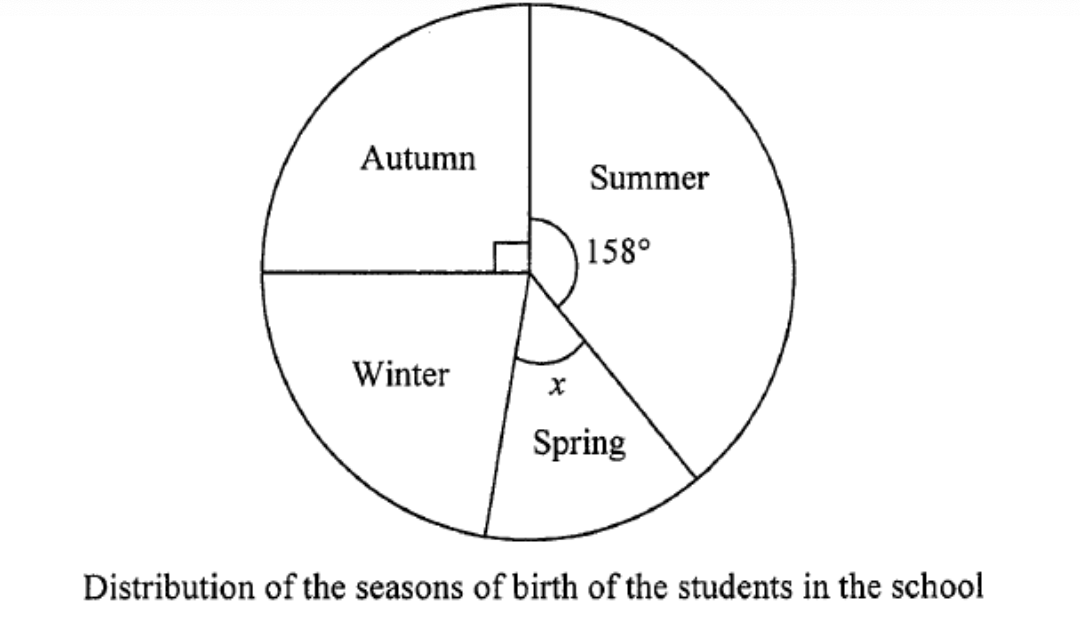
\includegraphics[width = .3\linewidth]{2017Figure1.00}
	\end{figure}
	If a student is randomly selected from the school, then the probability that the selected student was born in spring is $\dfrac{1}{9}$.
	\begin{enumerate}
		\item[(a)] Find $x$.
		\item[(b)] In the school, there are 180 students born in winter. Find the number of students in the school.
	\end{enumerate}
	(4 marks)
	
	\item \textbf{HKDSE MATH CORE 2017 Past Paper I Q8}\\
	It is given that $y$ varies inversely as $\sqrt{x}$. When $x = 144, y = 81$.
	\begin{enumerate}
		\item[(a)] Express $y$ in terms of $x$.
		\item[(b)] If the value of $x$ is increased from 144 to 324, find the change in the value of $y$.
	\end{enumerate}
	(5 marks)	
	
	\item \textbf{HKDSE MATH CORE 2017 Past Paper I Q9}\\
	A bottle is termed standard if its capacity is measured as 200 mL correct to the nearest 10 mL.
	\begin{enumerate}
		\item[(a)] Find the least possible capacity of a standard bottle.
		\item[(b)] Someone claims that the total capacity of 120 standard bottles can be measured as 23.3 L correct to the nearest 0.1 L. Do you agree? Explain your answer.
	\end{enumerate}
	(5 marks)

	\item \textbf{HKDSE MATH CORE 2017 Past Paper I Q10}\\
	In Figure 1, $OPQR$ is a quadrilateral such that $OP = OQ = OR$. $OQ$ and $PR$ intersect at the point $S$. $S$ is the mid-point of $PR$.
	\begin{figure}[H]
		\centering
		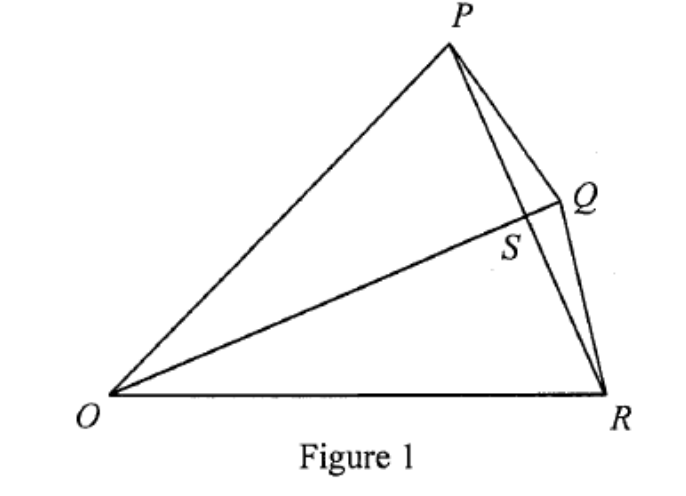
\includegraphics[width = .3\linewidth]{2017Figure1.1}
	\end{figure}
	\begin{enumerate}
		\item[(a)] Prove that $\triangle OPS \equiv \triangle ORS$. \\(2 marks)
		\item[(b)] It is given that $o$ is the centre of the circle which passes through $P$, $Q$ and $R$. If $OQ$ = 6 cm and $\angle PRQ = 10^\circ$, find the area of the sector $OPQR$ in terms of $\pi$. \\(4 marks)
	\end{enumerate}

	\item \textbf{HKDSE MATH CORE 2017 Past Paper I Q11}\\
	The stem-and-leaf diagram below shows the distribution of the hourly wages (in dollars) of the workers in a group.
	\begin{table}[htbp]
		\centering
		\begin{tabular}{r|l@{\hspace{4 pt}}l@{\hspace{4 pt}}l@{\hspace{4 pt}}l@{\hspace{4 pt}}}
		   Stem (tens) & Leaf (units)     \\
			\hline
			6     & 1 1 1 3 4 6 8 9 9\\    
			7     & $a$ 7 7 8\\    
			8     & 1 $b$\\    
		\end{tabular}
	\end{table}
	It is given that the mean and the range of the above distribution are \$70 and \$22 respectively.
	\begin{enumerate}
		\item[(a)] Find the median and the standard deviation of the above distribution. \\(5 marks)
		\item[(b)] If a worker is randomly selected from the group, find the probability that the hourly wage of the selected worker exceeds \$70. \\(2 marks)
	\end{enumerate}

	\item \textbf{HKDSE MATH CORE 2017 Past Paper I Q12}\\
	A solid metal right prism of base area 84 cm2 and height 20 cm is melted and recast into two similar solid right pyramids. The bases of the two pyramids are squares. The ratio of the base area of the smaller pyramid to the base area of the larger pyramid is 4 : 9.
	\begin{enumerate}
		\item[(a)] Find the volume of the larger pyramid. \\(3 marks)
		\item[(b)] If the height of the larger pyramid is 12 cm, find the total surface area of the smaller pyramid. \\(4 marks)
	\end{enumerate}

	\item \textbf{HKDSE MATH CORE 2017 Past Paper I Q13}\\
	The coordinates of the points $E$, $F$ and $G$ are $(-6, 5)$, $(-3, 11)$ and $(2, -1)$ respectively. The circle $C$ passes through $E$ and the centre of $C$ is $G$.
	\begin{enumerate}
		\item[(a)] Find the equation of $C$. \\(2 marks)
		\item[(b)] Prove that $F$ lies outside $C$. \\(2 marks)
		\item[(c)] Let $H$ be a moving point on $C$. When $H$ is farthest from $F$,
		\begin{enumerate}
			\item[(i)] describe the geometric relationship between $F$, $G$ and $H$;
			\item[(ii)] find the equation of the straight line which passes through $F$ and $H$.
		\end{enumerate}
		(3 marks)
	\end{enumerate}

	\item \textbf{HKDSE MATH CORE 2017 Past Paper I Q14}\\
	Let $f(x) = 6x^3 - 13x^2 - 46x + 34$. When $f(x)$ is divided by $2x^2 + ax + 4$, the quotient and the remainder are $3x + 7$ and $bx + c$ respectively, where $a$, $b$ and $c$ are constants.
	\begin{enumerate}
		\item[(a)] Find $a$. \\(3 marks)
		\item[(b)] Let $g(x)$ be a quadratic polynomial such that when $g(x)$ is divided by $2x^2 + ax + 4$, the remainder is $bx + c$.
		\begin{enumerate}
			\item[(i)] Prove that  $f(x) - g(x)$ is divisible by $2x^2 + ax + 4$.
			\item[(ii)] Someone claims that all the roots of the equation  $f(x) - g(x) = 0$ are integers. Do you agree? Explain your answer.
		\end{enumerate}
		(5 marks)
	\end{enumerate}

	\item \textbf{HKDSE MATH CORE 2017 Past Paper I Q15}\\
	Let $a$ and $b$ be constants. Denote the graph of $y = a + \log_b{x}$ by $G$. The $x$-intercept of $G$ is 9 and $G$ passes through the point $(243, 3)$ Express $x$ in terms of $y$. \\(4 marks)

	\item \textbf{HKDSE MATH CORE 2017 Past Paper I Q16}\\
	A city adopts a plan to import water from another city. It is given that the volume of water imported in the 1st year since the start of the plan is $1.5 \times 107$ m$^3$ and in subsequent years, the volume of water imported each year is 10\% less than the volume of water imported in the previous year.
	\begin{enumerate}
		\item[(a)] Find the total volume of water imported in the first 20 years since the start of the plan. \\(2 marks) 
		\item[(b)] Someone claims that the total volume of water imported since the start of the plan will not exceed $1.6 \times 108$ m$^3$. Do you agree? Explain your answer. \\(2 marks)
	\end{enumerate}

	\item \textbf{HKDSE MATH CORE 2017 Past Paper I Q17}\\
	In a bag, there are 4 green pens, 7 blue pens and 8 black pens. If 5 pens are randomly drawn from the bag at the same time,
	\begin{enumerate}
		\item[(a)] find the probability that exactly 4 green pens are drawn; \\(2 marks)
		\item[(b)] find the probability that exactly 3 green pens are drawn; \\(2 marks)
		\item[(c)] find the probability that not more than 2 green pens are drawn. \\(2 marks)
	\end{enumerate}

	\item \textbf{HKDSE MATH CORE 2017 Past Paper I Q18}\\
	The equation of the parabola $\Gamma$ is $2x^2 - 2kx + 2x - 3k + 8$, where $k$ is a real constant. Denote the straight line $y = 19$ by $L$.
	\begin{enumerate}
		\item[(a)] Prove that $L$ and $\Gamma$ intersect at two distinct points. \\(3 marks)
		\item[(b)] The points of intersection of $L$ and $\Gamma$ are $A$ and $B$.
		\begin{enumerate}
			\item[(i)] Let $a$ and $b$ be the $x$-coordinates of $A$ and $B$ respectively. Prove that $(a - b)^2 = k^2 + 4k + 23$.
			\item[(ii)] Is it possible that the distance between $A$ and $B$ is less than 4? Explain your answer.
		\end{enumerate}
		(5 marks)
	\end{enumerate}

	\item \textbf{HKDSE MATH CORE 2017 Past Paper I Q19}\\
	$ABC$ is a thin triangular metal sheet, where $BC = 24$ cm, $\angle BAC = 30^\circ$ and $\angle ACB = 42^\circ$.	
	\begin{enumerate}
		\item[(a)] Find the length of $AC$. \\(2 marks)
		\item[(b)] In Figure 2, the thin metal sheet $ABC$ is held such that only the vertex $B$ lies on the horizontal ground. $D$ and $E$ are points lying on the horizontal ground vertically below vertices $A$ and $C$ respectively. $AC$ produced meets the horizontal ground at the point $F$. A craftman finds that $AD = 10$ cm and $CE = 2$ cm.
		\begin{figure}[H]
			\centering
			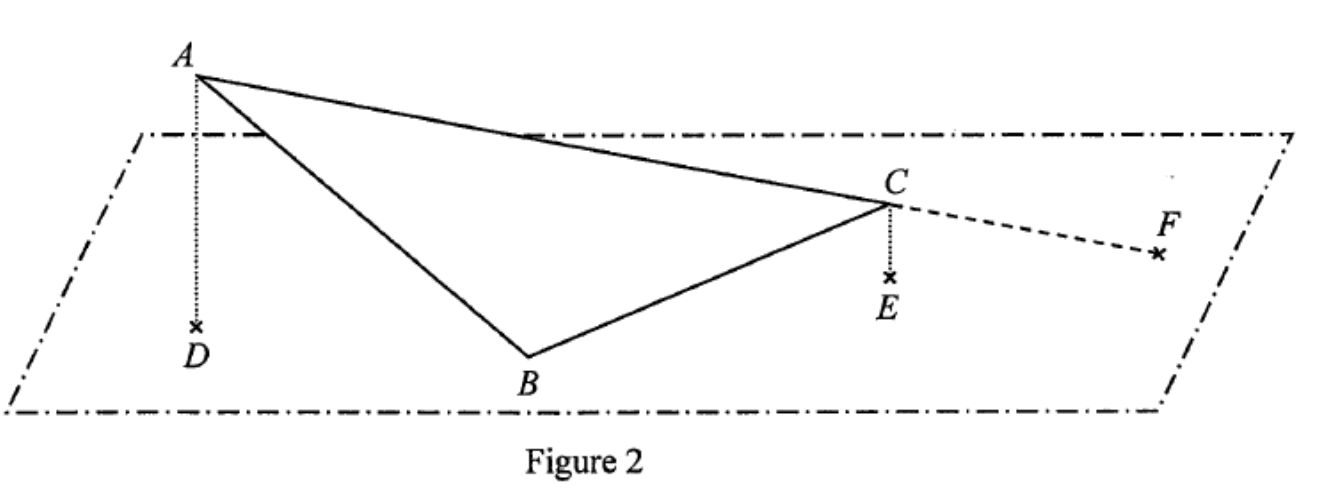
\includegraphics[width = .3\linewidth]{2017Figure1.2}
		\end{figure}
		\begin{enumerate}
			\item[(i)] Find the distance between $C$ and $F$.
			\item[(ii)] Find the area of $\triangle ABF$.
			\item[(iii)] Find the inclination of the thin metal sheet $ABC$ to the horizontal ground.
			\item[(iv)] The craftman claims that the area of $\triangle BDF$ is greater than 460 cm$^2$. Do you agree? Explain your answer.
		\end{enumerate}
		(11 marks)
	\end{enumerate}


\end{enumerate}
\end{document}